\documentclass[12pt]{article}

% Packages
\usepackage[utf8]{inputenc}  % Encoding
\usepackage[T1]{fontenc}     % Font encoding
\usepackage{lmodern}         % Improved font rendering
\usepackage{amsmath}         % Math symbols
\usepackage{amsfonts}        % Math fonts
\usepackage{amssymb}         % Additional math symbols
\usepackage{graphicx}        % Include graphics
\usepackage{hyperref}        % Hyperlinks
\usepackage{geometry}        % Page layout
\geometry{a4paper, margin=1in}

% Title, author, and date
\title{Numerically Solving Navier Stokes equation with GPUs}
\author{Gašper Golob}
\date{\today}

\begin{document}

% Title
\maketitle

% Introduction
\section{Introduction}
The goal of the project is to use the GPU to accelerate the execution of some methods for 
solving the Navier Stokes equation. Specifically the two methods that are being accelerated are 
variants of the artificial compressibility method.

The methods work iteratively, where at each time step, they compute new velocities using the 
Navier Stokes equation. Afterwards they correct the pressure using the assumed pressure volume 
invariant. 

For the purposes of this project the details of solving the partial differential equations are not 
as important, because the project is mostly concerned with accelerating the solving of systems and 
various matrix operations.

The GPU versions are also compared to their base versions to gauge the level of improvement and to 
see if they are still accurate.

The project is made using C++, where the discretization of the differential equations is done using 
the medusa library \cite{medusa}. To solve linear systems and work with matrices on the CPU the 
Eigen library is used. Similarly, to work with matrices on the GPU CUDA libraries such as
cuSolver, cuSparse and cuDSS are used.
\section{Implicit method}
For the implicit version of the method we are mostly concerned with solving two linear systems.
The first system involves solving using a system using the matrix \(M_u\). This matrix changes on 
every time step, so we need a solver, that can quickly solve a different system on each step.

The other system solves a system with the matrix \(M_p\), which remains unchanged between different 
iterations. This system is solved up to 100 times per time step, so it makes sense to preprocess the 
matrix for faster solving.

The comparison of times can be seen on figure \ref{fig:lidDriven_time}. On the graph we are comparing 
the base CPU implementation denoted with lid driven cavity with other variants.

The first variant lid driven cavity QR GPU uses the cusolverSp function cusolverSpDcsrlsvqr to 
solve the \(M_u\) system. We can see it starts of slower than the CPU version, but quickly becomes
faster.

The second variant solves the \(M_u\) system using the cuDSS library which contains 
functions for directly solving sparse systems. It uses a form of sparse LU decomposition, to solve
the linear system. As we can see from the graph this function gave the best speedup among all available.

The last variant lid driven cavity GPU with DSS and RF attempts to speed up the second linear system 
\(M_p\). This is done using the cusparseRF cuda library, which takes as input a sparseLU decomposition 
and uses it to solve a linear system. The LU factorization still has to be done on the CPU, 
as CUDA currently lacks GPU based functions for this. We see that this version is not faster than 
the previous version that simply accelerates the solving of the \(M_u\) system using the cuDSS library.
This is likely because the solving of the systems using the LU decomposition does not contain enough
parallelism, which means that the CPU version with the better single threaded performance is faster.
\begin{figure}[h!] 
    \centering 
    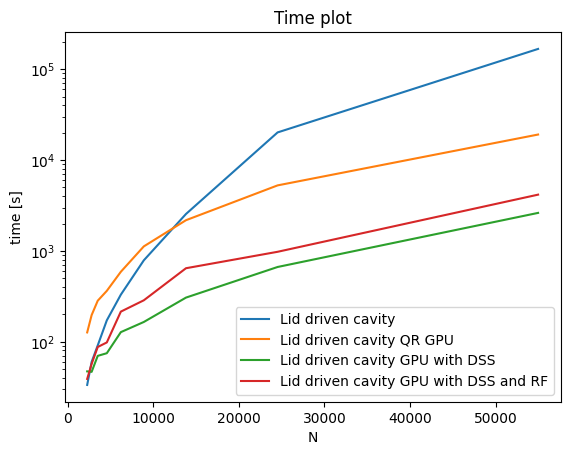
\includegraphics[width=0.8\textwidth]{lidDriven_time.png} 
    \caption{Graph of times to simulate 50 seconds of the lid driven cavity problem, 
    for different problem sizes.} 
    \label{fig:lidDriven_time} 
\end{figure}
\section{Explicit method}
% References
\begin{thebibliography}{99}
    \bibitem{medusa} Jure Slak and Gregor Kosec. 2021. Medusa: A C++ Library
    for Solving PDEs Using Strong Form Mesh-free Methods. ACM Trans. Math. Softw. 47,
    3, Article 28 (September 2021), 25 pages. https://doi.org/10.1145/3450966
\end{thebibliography}

\end{document}
